\clearpage
\setcounter{page}{1}
\cfoot{}
%\cfoot{陳立教育 -答案卷\thepage- 絕對智慧 }%中間 footer 擺放頁碼
%\input{AnswerPage.tex}
%\newpage
\clearpage
\setcounter{page}{1}
\cfoot{陳立教育 -解\thepage- 絕對智慧 }%中間 footer 擺放頁碼
%詳解區抬頭
% !TEX encoding = UTF-8 Unicode
% !TEX TS-program = xelatex
%詳解區抬頭
\psset{cornersize=absolute,linearc=.5\baselineskip} 
\psframebox[framesep=10pt]
{		
    \begin{minipage}[c]{16cm}
        {
            \fontsize{22}{22}
            \makebox[\textwidth][s]{\ChenLi \classNameString \yearString  \numForQuizTitle } \par  
           }
    \end{minipage}
}

%正式詳解區:
\def\FlagShowAnswer{1}  %設定顯現 QANS environment 裡面的資料
\def\FlagShowSolution{1} %設定顯現 QSOL environment 裡面的資料
\def\FlagAddSolutionBox{0}
%設定三大題區塊

\vspace{1cm}

\titleonetopic
% !TEX encoding = UTF-8 Unicode
% !TEX TS-program = xelatex 
\begin{QUESTIONS}
    \begin{QUESTION}
        \begin{ExamInfo}{106}{學測}{單選}{1}
        \end{ExamInfo}
        \begin{QBODY}
            已知某校老師玩過「寶可夢」的比率為${{r}_{1}}$,而學生玩過的比率為${{r}_{2}}$,其中${{r}_{1}}\ne {{r}_{2}}$。
        由下列選項中的資訊,請選出可以判定全校師生玩過「寶可夢」的比率之選項。
        \begin{QOPS}
            \QOP 全校老師與學生比率     
            \QOP 全校老師人數
            \QOP 全校學生人數
            \QOP 全校師生人數
            \QOP 全校師生玩過「寶可夢」人數
        \end{QOPS}
        \end{QBODY}
        \begin{QFROMS}
        \end{QFROMS}
        \begin{QTAGS}
        \end{QTAGS}
        \begin{QANS}
            (1)
        \end{QANS}
        \begin{QSOL}
        \end{QSOL}
        \begin{QEMPTYSPACE}
        \end{QEMPTYSPACE}
    \end{QUESTION}
    \begin{QUESTION}
        \begin{ExamInfo}{106}{學測}{單選}{2}
        \end{ExamInfo}
        \begin{QBODY}
            某個手機程式,每次點擊螢幕上的數$a$後,螢幕上的數會變成${{a}^{2}}$。當一開始時螢幕上的數$b$為正且連續點擊螢幕三次後,螢幕上的數接近${{81}^{3}}$。試問實數$b$最接近下列哪一個選項?
        \begin{QOPS}
            \QOP $1.7$      
            \QOP $3$      
            \QOP $5.2$      
            \QOP $9$      
            \QOP $81$
        \end{QOPS}
        \end{QBODY}
        \begin{QFROMS}
        \end{QFROMS}
        \begin{QTAGS}
        \end{QTAGS}
        \begin{QANS}
            (3)
        \end{QANS}
        \begin{QSOL}
        \end{QSOL}
        \begin{QEMPTYSPACE}
        \end{QEMPTYSPACE}
    \end{QUESTION}
    \begin{QUESTION}
        \begin{ExamInfo}{106}{學測}{單選}{3}
        \end{ExamInfo}
        \begin{QBODY}
            設$\Gamma :\frac{{{y}^{2}}}{{{a}^{2}}}-\frac{{{x}^{2}}}{{{b}^{2}}}=1$為坐標平面上一雙曲線,且其通過第一象限的漸近線為$\ell $。考慮動點$(t,{{t}^{2}})$,從時間$t=0$時出發。當$t>0$時,請選出正確的選項。
        \begin{QOPS}
        \QOP 此動點不會碰到$\Gamma $,也不會碰到$\ell $
        \QOP 此動點會碰到$\Gamma $,但不會碰到$\ell $
        \QOP 此動點會碰到$\ell $,但不會碰到$\Gamma $
        \QOP 此動點會先碰到$\Gamma $,再碰到$\ell $
        \QOP 此動點會先碰到$\ell $,再碰到$\Gamma $
        \end{QOPS}
        \end{QBODY}
        \begin{QFROMS}
        \end{QFROMS}
        \begin{QTAGS}
        \end{QTAGS}
        \begin{QANS}
            (5)
        \end{QANS}
        \begin{QSOL}
        \end{QSOL}
        \begin{QEMPTYSPACE}
        \end{QEMPTYSPACE}
    \end{QUESTION}
    \begin{QUESTION}
        \begin{ExamInfo}{106}{學測}{單選}{4}
        \end{ExamInfo}
        \begin{QBODY}
            在右下圖的正立方體上有兩質點分別自頂點$A,C$同時出發,各自以等速直線運動分別向頂點$B,D$前進,且在1秒後分別同時到達$B,D$。請選出這段時間兩質點距離關係的正確選項。
        
        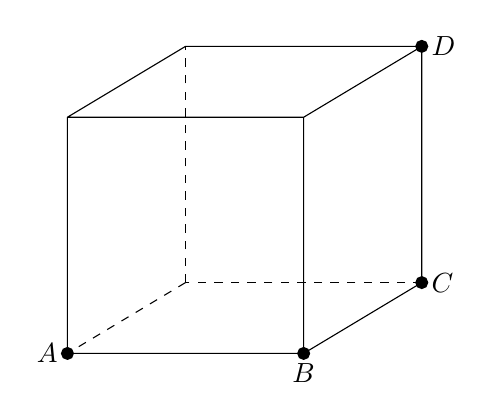
\begin{tikzpicture}[every edge quotes/.append style={auto, text=blue},
        x={(-0.25cm,-0.15cm)},
        y={(0.5cm,0cm)},
        z={(0cm,0.5cm)}]
        %%空間坐標中的CUBE 是以平面上的x軸 y軸再去擴充出深度z軸 z 往前為正,向後為負
        \coordinate (O) at (0,0,0);
        \coordinate (x) at (7,0,0);
        \coordinate (y) at 
        (0,7,0);
        \coordinate (z) at (0,0,7);
        
        \coordinate (Base1) at (0,0,0);
        \coordinate (Base2) at (6,0,0);
        \coordinate (Base3) at (6,6,0);
        \coordinate (Base4) at (0,6,0);
        \coordinate (Base1Up) at (0,0,6);
        \coordinate (Base2Up) at (6,0,6);
        \coordinate (Base3Up) at (6,6,6);
        \coordinate (Base4Up) at (0,6,6);
        
        \coordinate (A) at (Base2);
        \coordinate (B) at (Base3);
        \coordinate (C) at (Base4);
        \coordinate (D) at (Base4Up);
        
        \draw [draw=black, every edge/.append style={draw=black, dashed}]
        (Base1) edge (Base2)
        (Base2) -- (Base3)
        (Base3) -- (Base4)
        (Base4) edge (Base1)
        (Base1Up) -- (Base2Up)
        (Base2Up) -- (Base3Up)
        (Base3Up) -- (Base4Up)
        (Base4Up) -- (Base1Up)
        (Base1) edge (Base1Up)
        (Base2) -- (Base2Up)
        (Base3) -- (Base3Up)
        (Base4) -- (Base4Up);
        
        \foreach \v/\u/\t in 
        { A/left/$A$,
            B/below/$B$,
            C/right/$C$,
            D/right/$D$
        }
        {
            \draw[ultra thick,fill] (\v) circle (1.5pt);
            \node[\u] at (\v){\t};
        }; 
        
        \end{tikzpicture}
        
        \begin{QOPS}
            \QOP 兩質點的距離固定不變
            \QOP 兩質點的距離越來越小
            \QOP 兩質點的距離越來越大
            \QOP 在$\frac{1}{2}$秒時兩質點的距離最小
            \QOP 在$\frac{1}{2}$秒時兩質點的距離最大
        \end{QOPS}
        \end{QBODY}
        \begin{QFROMS}
        \end{QFROMS}
        \begin{QTAGS}
        \end{QTAGS}
        \begin{QANS}
            (4)
        \end{QANS}
        \begin{QSOL}
        \end{QSOL}
        \begin{QEMPTYSPACE}
        \end{QEMPTYSPACE}
    \end{QUESTION}
    \begin{QUESTION}
        \begin{ExamInfo}{106}{學測}{單選}{5}
        \end{ExamInfo}
        \begin{QBODY}
            下圖是某城市在2016年的各月最低溫(橫軸$x$)與最高溫(縱軸$y$)的散佈圖。
        
        今以溫差(最高溫減最低溫)為橫軸且最高溫為縱軸重新繪製一散佈圖。試依此選出正確的選項。
        \begin{QOPS}
            \QOP 最高溫與溫差為正相關,且它們的相關性比最高溫與最低溫的相關性強
            \QOP 最高溫與溫差為正相關,且它們的相關性比最高溫與最低溫的相關性弱
            \QOP 最高溫與溫差為負相關,且它們的相關性比最高溫與最低溫的相關性強
            \QOP 最高溫與溫差為負相關,且它們的相關性比最高溫與最低溫的相關性弱
            \QOP 最高溫與溫差為零相關
        \end{QOPS}
        \end{QBODY}
        \begin{QFROMS}
        \end{QFROMS}
        \begin{QTAGS}
        \end{QTAGS}
        \begin{QANS}
            (4)
        \end{QANS}
        \begin{QSOL}
        \end{QSOL}
        \begin{QEMPTYSPACE}
        \end{QEMPTYSPACE}
    \end{QUESTION}
    \begin{QUESTION}
        \begin{ExamInfo}{106}{學測}{單選}{6}
        \end{ExamInfo}
        \begin{QBODY}
            試問有多少個實數$x$滿足$\frac{\pi }{2}\le x\le \frac{3\pi }{2}$且$\cos x{}^\circ \le \cos x$?
        \begin{QOPS}
            \QOP $0$個     
            \QOP $1$個     
            \QOP $2$個     
            \QOP $4$個     
            \QOP 無窮多個
        \end{QOPS}
        \end{QBODY}
        \begin{QFROMS}
        \end{QFROMS}
        \begin{QTAGS}
        \end{QTAGS}
        \begin{QANS}
        \end{QANS}
        \begin{QSOL}
        \end{QSOL}
        \begin{QEMPTYSPACE}
        \end{QEMPTYSPACE}
    \end{QUESTION}
    \begin{QUESTION}
        \begin{ExamInfo}{106}{學測}{單選}{7}
        \end{ExamInfo}
        \begin{QBODY}
            小明想要安排從星期一到星期五共五天的午餐計畫。他的餐點共有四種選擇:牛肉麵、大滷麵、咖哩飯及排骨飯。小明想要依據下列兩原則來安排他的午餐:
        (甲)每天只選一種餐點但這五天中每一種餐點至少各點一次
        (乙)連續兩天的餐點不能重複且不連續兩天吃麵食
        根據上述原則,小明這五天共有幾種不同的午餐計畫?
        \begin{QOPS}
            \QOP $52$      
            \QOP $60$      
            \QOP $68$      
            \QOP $76$      
            \QOP $84$
        \end{QOPS}
        \end{QBODY}
        \begin{QFROMS}
        \end{QFROMS}
        \begin{QTAGS}
        \end{QTAGS}
        \begin{QANS}
            (2)
        \end{QANS}
        \begin{QSOL}
        \end{QSOL}
        \begin{QEMPTYSPACE}
        \end{QEMPTYSPACE}
    \end{QUESTION}

\end{QUESTIONS}
\newpage
\titletwotopic
% !TEX encoding = UTF-8 Unicode
% !TEX TS-program = xelatex
\begin{QUESTIONS}
	\setcounter{enumi}{8}
\begin{QUESTION}
    \begin{QBODY}	設$m,n$為小於或等於4的相異正整數且$a,b$為非零實數。已知函數$f(x)=a{{x}^{m}}$與函數$g(x)=b{{x}^{n}}$的圖形恰有3個相異交點,請選出可能的選項。
        \begin{QOPS}
        \QOP $m,n$皆為偶數且$a,b$同號 
        \QOP $m,n$皆為偶數且$a,b$異號
        \QOP $m,n$皆為奇數且$a,b$同號
        \QOP $m,n$皆為奇數且$a,b$異號
        \QOP $m,n$為一奇一偶
        \end{QOPS}
    \end{QBODY}
    \begin{QFROMS}
    \end{QFROMS}
    \begin{QTAGS}
    \end{QTAGS}
    \begin{QANS}
        (1)(3)
    \end{QANS}
    \begin{QSOL}
    \end{QSOL}
    \begin{QEMPTYSPACE}
    \end{QEMPTYSPACE}
\end{QUESTION}
\begin{QUESTION}
    \begin{QBODY}
        設$\Gamma $為坐標平面上的圓,點$(0,0)$在$\Gamma $的外部且點$(2,6)$在$\Gamma $的內部。請選出正確的選項。
        \begin{QOPS}
        \QOP $\Gamma $的圓心不可能在第二象限
        \QOP $\Gamma $的圓心可能在第三象限且此時$\Gamma $的半徑必定大於10
        \QOP $\Gamma $的圓心可能在第一象限且此時$\Gamma $的半徑必定小於10
        \QOP $\Gamma $的圓心可能在$x$軸上且此時圓心的$x$坐標必定小於10
        \QOP $\Gamma $的圓心可能在第四象限且此時$\Gamma $的半徑必定大於10
        \end{QOPS}
    \end{QBODY}
    \begin{QFROMS}
    \end{QFROMS}
    \begin{QTAGS}
    \end{QTAGS}
    \begin{QANS}
        (5)
    \end{QANS}
    \begin{QSOL}
    \end{QSOL}
    \begin{QEMPTYSPACE}
    \end{QEMPTYSPACE}
\end{QUESTION}
\begin{QUESTION}
    \begin{QBODY}
        坐標空間中有三直線${{L}_{1}}:\dfrac{x-1}{2}=\dfrac{y+1}{2}=\dfrac{z}{1},{{L}_{2}}:\left\{ \begin{aligned}
        & x-2y+2z=-4 \\ 
        & x+y-4z=5 \\ 
        \end{aligned} \right.,{{L}_{3}}:\left\{ \begin{aligned}
        & x=-t \\ 
        & y=-2-t \\ 
        & z=4+4t \\ 
        \end{aligned} \right.$,$t$為實數。請選出正確的選項。
        \begin{QOPS}
            \QOP ${{L}_{1}}$與${{L}_{2}}$的方向向量互相垂直
            \QOP ${{L}_{1}}$與${{L}_{3}}$的方向向量互相垂直
            \QOP 有一個平面同時包含${{L}_{1}}$與${{L}_{2}}$
            \QOP 有一個平面同時包含${{L}_{1}}$與${{L}_{3}}$
            \QOP 有一個平面同時包含${{L}_{2}}$與${{L}_{3}}$
        \end{QOPS}
    \end{QBODY}
    \begin{QFROMS}
    \end{QFROMS}
    \begin{QTAGS}
    \end{QTAGS}
    \begin{QANS}
        (2)(3)(4)
    \end{QANS}
    \begin{QSOL}
    \end{QSOL}
    \begin{QEMPTYSPACE}
    \end{QEMPTYSPACE}
\end{QUESTION}
\begin{QUESTION}
    \begin{QBODY}
        設最近數學家發現一種新的可以無縫密舖平面的凸五邊形$ABCDE$,其示意圖如下。關於這五邊形,請選出正確的選項。
        
        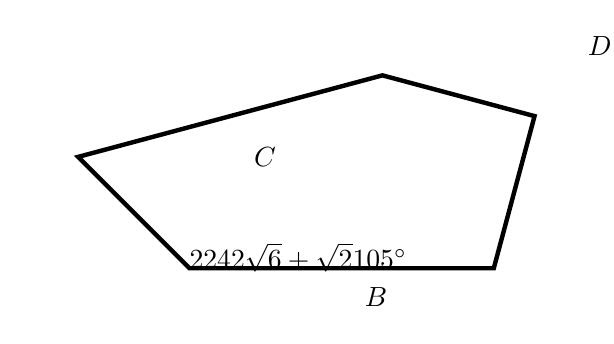
\begin{tikzpicture}[scale=1.0]
        
        \coordinate (B) at (0,0);
        \coordinate (A) at (0:{sqrt(6)+sqrt(2)});
        \path (A) ++(75:2) coordinate (E);
        \path (E) ++(165:2) coordinate (D);
        \coordinate (C) at (135:2);
        
        
        \draw[ultra thick] (A) -- (B)--(C)--(D)--(E) --cycle;
        \tkzLabelSegment[midway,  right](E,A){$2$};
        \tkzLabelSegment[midway,  above](D,E){$2$};
        \tkzLabelSegment[midway,  above](D,C){$4$};
        \tkzLabelSegment[midway,  below left](C,B){$2$};
        \tkzLabelSegment[midway,  below](B,A){$\sqrt{6}+\sqrt{2}$};
        \tkzMarkRightAngle[size=0.3](D,E,A);
        \tkzMarkAngle[size=0.3](E,A,B);
        \tkzLabelAngle[pos=0.6](E,A,B){$105^\circ$};
        
        \node[label=315:$A$] at (A){};
        \node[label=225:$B$] at (B){};
        \node[label=180:$C$] at (C){};
        \node[label=90:$D$] at (D){};
        \node[label=45:$E$] at (E){};
        \end{tikzpicture}
        \begin{QOPS}
        \QOP $\overline{AD}=2\sqrt[{}]{2}$
        \QOP $\angle DAB=45{}^\circ $
        \QOP $\overline{BD}=2\sqrt[{}]{6}$
        \QOP $\angle ABD=45{}^\circ $
        \QOP $BCD$的面積為$2\sqrt[{}]{2}$
        \end{QOPS}
    \end{QBODY}
    \begin{QFROMS}
    \end{QFROMS}
    \begin{QTAGS}
    \end{QTAGS}
    \begin{QANS}
        (1)(4)
    \end{QANS}
    \begin{QSOL}
    \end{QSOL}
    \begin{QEMPTYSPACE}
    \end{QEMPTYSPACE}
\end{QUESTION}
\begin{QUESTION}
    \begin{QBODY}
        某班級50位學生,段考國文、英文、數學及格的人數分別為45、39、34人,且英文及格的學生國文也都及格。現假設數學和英文皆及格的有$x$人,數學及格但英文不及格的有$y$人。請選出正確的選項。
        \begin{QOPS}
            \QOP $x+y=39$
            \QOP $y\le 11$
            \QOP 三科中至少有一科不及格的學生有$39-x+y$人
            \QOP 三科中至少有一科不及格的學生最少有11人
            \QOP 三科中至少有一科不及格的學生最多有27人
        \end{QOPS}
    \end{QBODY}
    \begin{QFROMS}
    \end{QFROMS}
    \begin{QTAGS}
    \end{QTAGS}
    \begin{QANS}
        (2)(5)
    \end{QANS}
    \begin{QSOL}
        \begin{QSTEPS}
            \QSTEP{ 令全班為集合$U$,國文、數學、英文,及格的集合分別為 $C,M,E$ \\
                    可得:$n(C) = 45, n(M) = 34 , n(E) = 39$}
            \QSTEP{ $x+y = n (M \cap E) + n (M \cap \overline{E}) = n(M) = 34$,則 (1) 錯誤}
            \QSTEP{ $n(\bar{E}) = 50 -39 =11 \ge n (M \cap \bar{E}) \Rightarrow y \le 11$,則 (2) 正確}
            \QSTEP{ 由以上兩步驟可得 $23 \le x\le 34$}
            \QSTEP{ 至少一科不及格 $= n(\text{全}) - n (C\cap M\cap E) = 50-x$,\\
                    可得 $16 \le \text{至少一科不及格} \le 27$}
        \end{QSTEPS}
        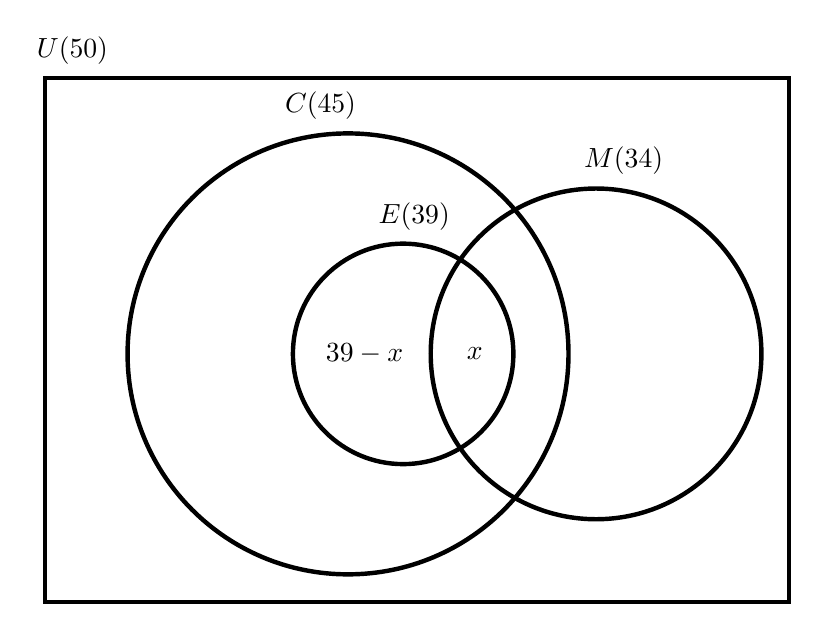
\begin{tikzpicture}[scale=0.7]
            \draw[ultra thick]  (-6.5,6) circle (2);
            \draw[ultra thick]  (-7.5,6) node (v1) {} ellipse (4 and 4);
            
            
            \draw[ultra thick]  (-3,6) node (v2) {} circle (3);
            
            \draw[ultra thick]  (-13,11) rectangle (0.5,1.5);
            
            \node at (-12.5,11.5) {$U(50)$};
            \node at (-8,10.5) {$C(45)$};
            
            \node at (-5.2,6) {$x$};
            
            \node at (-7.2,6) {$39-x$};
            \node at (-6.3,8.5) {$E(39)$};
            
            \node at (-2.5,9.5) {$M(34)$};
    \end{tikzpicture}
    \end{QSOL}
    \begin{QEMPTYSPACE}
    \end{QEMPTYSPACE}
\end{QUESTION}
\begin{QUESTION}
    \begin{QBODY}
        空間中有一四面體$ABCD$。假設$\lvec{AD}$分別與$\lvec{AB}$和$\lvec{AC}$垂直,請選出正確的選項。
        \begin{QOPS}
            \QOP $\lvec{DB}\cdot\lvec{DC} ={{\overline{DA}}^{2}}- \lvec{AB}\cdot \lvec{AC}$
            \QOP 若$\angle BAC$是直角,則$\angle BDC$是直角
            \QOP 若$\angle BAC$是銳角,則$\angle BDC$是銳角
            \QOP 若$\angle BAC$是鈍角,則$\angle BDC$是鈍角
            \QOP 若$\overline{AB}<\overline{DA}$且$\overline{AC}<\overline{DA}$,則$\angle BDC$是銳角
        \end{QOPS}
    \end{QBODY}
    \begin{QFROMS}
    \end{QFROMS}
    \begin{QTAGS}
    \end{QTAGS}
    \begin{QANS}
        (3)(5)
    \end{QANS}
    \begin{QSOL}
    \end{QSOL}
    \begin{QEMPTYSPACE}
    \end{QEMPTYSPACE}
\end{QUESTION}
\end{QUESTIONS}
\newpage
\setcounter{BLANKcounter}{\BLANKSTART}
\titlethreetopic
% !TEX encoding = UTF-8 Unicode
% !TEX TS-program = xelatex
%正式題目區:
%新增題目範本
%\begin{QUESTION}
%    \begin{QBODY}
%    \end{QBODY}
%    \begin{QFROMS}
%    \end{QFROMS}
%    \begin{QTAGS}
%    \end{QTAGS}
%    \begin{QANS}
%    \end{QANS}
%    \begin{QSOL}
%    \end{QSOL}
%    \begin{QEMPTYSPACE}
%    \end{QEMPTYSPACE}
%\end{QUESTION}
\begin{QUESTIONS}[label=$\Alph*.$]
\begin{QUESTION}
    \begin{QBODY}
        遞迴數列$\langle {{a}_{n}}\rangle $滿足${{a}_{n}}={{a}_{n-1}}+f(n-2)$,其中$n\ge 2$且$f(x)$為二次多項式。若${{a}_{1}}=1,{{a}_{2}}=2,{{a}_{3}}=5,{{a}_{4}}=12$,則${{a}_{5}}= \TCNBOX{ \TCN\TCN }$     。
        
    \end{QBODY}
    \begin{QFROMS}
    \end{QFROMS}
    \begin{QTAGS}
    \end{QTAGS}
    \begin{QANS}
        $25$
    \end{QANS}
    \begin{QSOL}
    \end{QSOL}
    \begin{QEMPTYSPACE}
    \end{QEMPTYSPACE}
\end{QUESTION}
\begin{QUESTION}
    \begin{QBODY}
         坐標平面上,$ABC$內有一點$P$滿足$\lvec{AP}=(\frac{4}{3},\frac{5}{6})$及$\lvec{AP}=\frac{1}{2}\lvec{AB}+\frac{1}{5}\lvec{AC}$。若$A,P$連線交$\overline{BC}$於$M$,則$\lvec{AM}= \TCNBOX{\left(\FR{\TCN\TCN}{\TCN\TCN} ,\FR{\TCN\TCN}{\TCN\TCN} \right)}$。(化成最簡分數)
    \end{QBODY}
    \begin{QFROMS}
    \end{QFROMS}
    \begin{QTAGS}
    \end{QTAGS}
    \begin{QANS}
        $(\frac{40}{21},\frac{25}{21})$
    \end{QANS}
    \begin{QSOL}
    \end{QSOL}
    \begin{QEMPTYSPACE}
    \end{QEMPTYSPACE}
\end{QUESTION}
\begin{QUESTION}
    \begin{QBODY}
        若$a$為正整數且方程式$5{{x}^{3}}+(a+4){{x}^{2}}+ax+1=0$的根都是有理根,則$a= \TCNBOX{\TCN}$     。
    \end{QBODY}
    \begin{QFROMS}
    \end{QFROMS}
    \begin{QTAGS}
    \end{QTAGS}
    \begin{QANS}
        $7$
    \end{QANS}
    \begin{QSOL}
    \end{QSOL}
    \begin{QEMPTYSPACE}
    \end{QEMPTYSPACE}
\end{QUESTION}
\begin{QUESTION}
    \begin{QBODY}
        設${{a}_{1}},{{a}_{2}},\cdots ,{{a}_{9}}$為等差數列且$k$為實數。若方程組
        $\left\{ \begin{aligned}
        & {{a}_{1}}x-{{a}_{2}}y+2{{a}_{3}}z=k+1 \\ 
        & {{a}_{4}}x-{{a}_{5}}y+2{{a}_{6}}z=-k-5 \\ 
        & {{a}_{7}}x-{{a}_{8}}y+2{{a}_{9}}z=k+9 \\ 
        \end{aligned} \right.$有解,
        則$k=\TCNBOX{\TCN\TCN}$      。
        
    \end{QBODY}
    \begin{QFROMS}
    \end{QFROMS}
    \begin{QTAGS}
    \end{QTAGS}
    \begin{QANS}
        $-5$
    \end{QANS}
    \begin{QSOL}
    \end{QSOL}
    \begin{QEMPTYSPACE}
    \end{QEMPTYSPACE}
\end{QUESTION}
\begin{QUESTION}
    \begin{QBODY}
        設$a,b,x$皆為正整數且滿足$a\le x\le b$及$b-a=3$。若用內插法從$\log a,\log b$求得$\log x$的
        近似值為
        $\log x\approx \frac{1}{3}\log a+\frac{2}{3}\log b=\frac{1}{3}(1+2\log 3-\log 2)+\frac{2}{3}(4\log 2+\log 3)$,
        則$x$的值為 $\TCNBOX{\TCN\TCN}$        。
        
    \end{QBODY}
    \begin{QFROMS}
    \end{QFROMS}
    \begin{QTAGS}
    \end{QTAGS}
    \begin{QANS}
        $47$
    \end{QANS}
    \begin{QSOL}
    \end{QSOL}
    \begin{QEMPTYSPACE}
    \end{QEMPTYSPACE}
\end{QUESTION}
\begin{QUESTION}
    \begin{QBODY}
         一隻青蛙位於坐標平面的原點,每步隨機朝上、下、左、右跳一單位長,總共跳了四步。青蛙跳了四步後恰回到原點的機率為$\TCNBOX{\FR{\TCN}{\TCN\TCN}}$。(化成最簡分數)
    \end{QBODY}
    \begin{QFROMS}
    \end{QFROMS}
    \begin{QTAGS}
    \end{QTAGS}
    \begin{QANS}
        $\frac{9}{64}$
    \end{QANS}
    \begin{QSOL}
    \end{QSOL}
    \begin{QEMPTYSPACE}
    \end{QEMPTYSPACE}
\end{QUESTION}
\begin{QUESTION}
    \begin{QBODY}
        地面上甲、乙兩人從同一地點同時開始移動。甲以每秒4公尺向東等速移動,乙以每秒3公尺向北等速移動。在移動不久之後,他們互望的視線被一圓柱體 建築物阻擋了6秒後才又相見。此圓柱體建築物底圓的直徑為$\TCNBOX{\TCN\TCN.\TCN}$公尺。
    \end{QBODY}
    \begin{QFROMS}
    \end{QFROMS}
    \begin{QTAGS}
    \end{QTAGS}
    \begin{QANS}
        $14.4$
    \end{QANS}
    \begin{QSOL}
    \end{QSOL}
    \begin{QEMPTYSPACE}
    \end{QEMPTYSPACE}
\end{QUESTION}
\end{QUESTIONS}

